\chapter{Implementation}
\label{sec:implementation}

% Hier greift man einige wenige, interessante Gesichtspunkte der
% Implementierung heraus. Das Kapitel darf nicht mit Dokumentation oder
% gar Programmkommentaren verwechselt werden. Es kann vorkommen, daß
% sehr viele Gesichtspunkte aufgegriffen werden müssen, ist aber nicht
% sehr häufig. Zweck dieses Kapitels ist einerseits, glaubhaft zu
% machen, daß man es bei der Arbeit nicht mit einem "Papiertiger"
% sondern einem real existierenden System zu tun hat. Es ist sicherlich
% auch ein sehr wichtiger Text für jemanden, der die Arbeit später
% fortsetzt. Der dritte Gesichtspunkt dabei ist, einem Leser einen etwas
% tieferen Einblick in die Technik zu geben, mit der man sich hier
% beschäftigt. Schöne Bespiele sind "War Stories", also Dinge mit denen
% man besonders zu kämpfen hatte, oder eine konkrete, beispielhafte
% Verfeinerung einer der in Kapitel 3 vorgestellten Ideen. Auch hier
% gilt, mehr als 20 Seiten liest keiner, aber das ist hierbei nicht so
% schlimm, weil man die Lektüre ja einfach abbrechen kann, ohne den
% Faden zu verlieren. Vollständige Quellprogramme haben in einer Arbeit
% nichts zu suchen, auch nicht im Anhang, sondern gehören auf Rechner,
% auf denen man sie sich ansehen kann.

% Implementation motivation

In section \ref{sec:design} the design of the communication library
was presented.  This section will pick up some details of the design
and how they were implemented during the developement of the
communication library. It will not be a full documentation of the
developed source code, this can be retrieved from the source code
or doxygen \cite{ref:doxygen} documentation itself.

The library started from the need of PIConGPU (Section \ref{sec:picongpu})
for a more flexibel and abstract communication layer. PIConGPU is implemented
in C++98 with additional usage of boost \cite{ref:boost} libraries. Thus
the communication library was also implemented in C++ but in the
ISO standard from 2011 \cite{ref:c++11}.



\section{The CAL with Policy Based Design}
  In section \ref{sec:cal} the Communication Abstraction Layer was
  introduced as an flexible Communication layer based on varying
  adapters. For the implementation of the varying adapters, a policy
  based design was choosen.

  % Policy based design in general
  A policy is a class or class template interface, which consists of
  inner type definitions, member functions and/or member variables. An
  implementation of a policy is called policy class and is inherited
  by or contained within a host class.  The advantage of policy based
  design is that the varying functionality of the policy is bounded to
  its host class at compile time, providing no runtime overhead. 
  The interface of the policy is strictly defined by the host
  class. Ignoring this interface leads to errors at compile time.

  % Policy based design for CAL + adapter
  In the CAL case, the adapter is the policy, here called
  communication policy, and the CAL is the host class (Figure
  \ref{fig:cal_uml}). The CAL takes an adapter as template argument
  and inheritates its properties in protected mode. The CAL provides
  all communication and context operations discussed in section
  \ref{sec:cal_context}. If these operations are adapter specific then
  they are forwarded to the adapters interface.

  % CAL provides interface, adapter has to implement this interface

  \begin{figure}[H]
    \centering 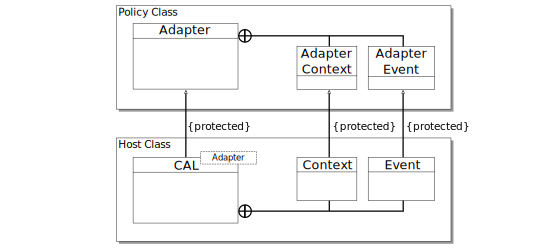
\includegraphics[width=\textwidth]{graphics/40_cal_uml}
    \caption{  }
    \label{fig:cal_uml}
  \end{figure}

  % Descrption Communication operations
  Usually, the adapter has to provide all communication and context
  operations. But, policy based design has the characteristic
  that if a member function not used through the host class, the
  compiler will not care if this function is implemented by the policy
  or not. Thus only the used member functions have to be implemented
  in an adapter (e.g just p2p functionality). But for sake of
  completeness an adapter should implement the whole policy interface.

  % Description Context + Event
  In addition to communication and context related member functions,
  the adapter has also to provide a inner context and a inner event
  class. Meaning and interface of these classes were explained in
  section \ref{sec:cal_comm}. Both contain the adapter specific
  implementations. The interface of these two inner classes is defined
  by according inner classes of the CAL and implanted by inheritance
  (Figure \ref{fig:cal_uml}.


\subsection{The MPI Adapter as Reference Implementation}
\label{sec:cal_mpi_adapter}
  The reference adapter implementation is based on MPI as existing
  communication layer.  MPI (Section \ref{sec:mpi}) was as choosen ,
  because it already brings a lot of functionality required by the CAL
  interface from the scratch. Additionally it is available on wide
  range of compute systems and can be used for free by open source
  implementations. To address the message passing interface, the MPI C
  language binding is used inside the adapter. An alternative would be
  the boost::mpi C++ implementation, which presupposes that beside a
  MPI implementation also the boost library is installed.

  Implementing the communication operation is straight forward, just a
  forwarding of arguments and a call to MPI. More tricky is the
  support of abitrary binary operations for the reduce operation and
  the support of abitrary data types of the trasmitted data.

  \begin{itemize}
  \item Binary Function

    A collective reduce operation is based on an binary operator. The
    CAL defined a very genral binary operator
    \ref{sec:cal_collective}. Thus it has to be specialized to a
    binary operator the adapter can handle. MPI supports binary
    operations, but they need to be transformed.  There exists two
    possible ways to do so. The easiest way, is that the MPI adapter
    provides all binary MPI functions by itself as kind of a struct
    with static const expressions (Listing \ref{lst:mpi_bin}). The CAL
    could forward this list of binary operators to the library user.

    \begin{lstlisting}[language=C++, caption={Binary operators by static constexpr.}, label=lst:mpi_bin]
      struct BinaryOperations { 	
        static constexpr BinaryOperation MAX = MPI_MAX; 	
        static constexpr BinaryOperation MIN = MPI_MIN; 	
        static constexpr BinaryOperation SUM = MPI_SUM; 	
        static constexpr BinaryOperation PROD = MPI_PROD;
	...
      };
    \end{lstlisting}

    The downside of the this approach is that only the predefined
    operations of MPI can be used. Of course there are more binary
    operations then the predefined ones. Therfore it is possible to
    create abitrary binary operators with MPI\_Op\_create, which can
    be done for all binary operators . The only requirement is that
    the binary operation has to be a struct like discussed in section
    \ref{sec:cal_collective}. This approach is essentially more flexible
    then the first approach. Thus it was chooses to implement binary
    operations for the MPI adapter.

  \item  Data Type Conversion 

    MPI predefines on one hand its primitive data types, but on the
    other hand also provides facilities to define own data structures
    based upon sequences of the MPI primitive data types. Such user
    defined structures are called derived data types. Primitive data
    types are contiguous. Derived data types allow you to specify
    non-contiguous data in a convenient manner and to treat it as
    though it was contiguous.

    The primitive c++ data types can be mapped directly to primitive
    C++ data types. The conversation is implemented by C++ traits .
    First, a generic template is defined that implements the default
    behaviour (Listing \ref{lst:mpi_trait1}). In this case unknown
    types will assumed to be of the MPI\_CHAR type. The second
    template is a specialisation for int, which will be transformed to
    MPI\_INT type (Listing \ref{lst:mpi_trait2}).


    \begin{lstlisting}[language=C++, label=lst:mpi_trait1]
      template<typename T>
      struct MPIDatatypes{
	static constexpr MPI_Datatype type = MPI_CHAR;
      };
    \end{lstlisting}

    \begin{lstlisting}[language=C++, label=lst:mpi_trait2]
      template<>
      struct MPIDatatypes<int>{
    	static constexpr MPI_Datatype type = MPI_INT;
      };

    \end{lstlisting}

    More complex data types (e.g structs or classes) have to be
    transformed into derived data types. This transformation is
    available in the boost::mpi implementation. Thus switching to
    boost::mpi \cite{ref:boost::mpi} would solve this problem without
    any further effort.

  \item MPI specific Context
  \item MPI specific Event
  \end{itemize}

\section{Graph Based on the Boost Graph Library}

  % BGL as backend
  The graph introduced in section \ref{sec:graph} was not written from
  the scratch. There are a varity of libraries providing graph
  implementations. Because of the closeness of the boost library to
  the C++ STL, the boost graph library \cite{ref:boost::bgl}, short
  BGL, was choosen. While the BGL provides a lot of functionality,
  just a small subset is really needed for the purposes of this
  work. Thus the BGL is wrapped inside a graph class just providing
  standard graph funcionality.



  \subsection{Vertices identified by Properties}

    % Properties
    Like in section \ref{sec:graph} discussed, a graph has so called
    properties that can be used to describe its vertices and
    edges. The BGL itself refers to vertices by integer numbers,
    whereby properties of this integer vertices can be queried from so
    called property maps. In this Graph, the vertices and edges are represented
    by its property itself and are configured at compile time.  The
    properties are structs or classes with abitrary content. However
    the properties need to provide an id member variable to create an
    internal connection of vertices to properties.  Thus asking for
    the vertices of the graph, returns a vector of vertices. That
    vector is a list of vertex properties in the context of the BGL,
    whereby every property is connected by its id to the graph.
  
  \subsection{Configuration of a Graph}
    The configuration of the graph requires two classes to define both
    vertex and edge property as template arguments.  If the graph
    should not contain any further information then the properties
    will be filled by default with a property only containing the id.

  \subsection{Creation of a Graph}
    A graph can be created by a list of edge descriptors and a list of
    vertices, while an edge descriptor is tuple of source vertex,
    destination vertex and the connecting edge. The vertices and edges
    can allready be filled with property information.  This list of
    edge descriptors can also generated by one of the several provided
    graph generators. These allow a generation of commonly used graph
    topologies.

    \todo{explain graph generators?}

  \subsection{Operations on the graph / vertices}
    % Operations
    The graph provides set of simple graph operations. Like retrieving all
    vertices, retrieving adjacent vertices, retrieving in and out
    edges.
    \todo{Is there more Information needed? Because it is not that interesting}

  \subsection{Creation of subgraphs}
    % Subgraph Createion
    Another reason for the BGL is the builtin subgraph support. The
    creation of subgraphs is meant to be used as an equivalent to the
    creation of contexts in the CAL. Thus a subgraph can be created from its
    supergraph by a subset of its vertices. Collective operations on
    this subgraph only consider vertices within this subgraph.

\subsection{Graph-based Virtual Overlay network}

\begin{itemize}
  \item Announce process
    In general, the announcement process is a collective operation of
    the peers that want to take part on the communication of a
    specific graph. These peers create first and foremost an exclusive
    context for themselves. Therfore the present context has to be
    determined. The most general context would be the global context
    of all peers in the network, but in some cases exists also a
    context with less peers. This is either the context of the graph,
    if it was allready announced, or the context of the supergraph.

    Afterwards a new context is created from the old one. This is done
    by a gather operation, while every peer declares the number of
    vertices it wants to announce. Every peer declaring zero vertices
    will not belong to the new context. The graph is finally mapped
    to the new context.

    The ids of the hosted vertices can now be exchanged by a further
    gather operation of the new context. Each peer updates now its
    vertex map for the graph by the retrieved vertex ids.

  \item Collective Operations locally

\end{itemize}

\subsection{Configuration and Initialization of an Application}

  Steps of Configuration

  \begin{enumerate}
  % Configuration
  \item Configure CAL 
  \item Configure graph with properties
  \item Configure virtual overlay network with graph and CAL

  % Initialization
  \item Create graph topologie
  \item Create CAL object and retrieve intial context
  \item Create virtual overlay network

  % Distribution and load balancing
  \item Distribute vertices of graph to peers of context
  \item Announce hosted vertices
  \end{enumerate}
  
\section{Implementing a Game of Life}
  
  % Introduction
  To show the communication library in a real world 
  application, Game of Life was implemented based on the developed
  communication library.

  % GoL Graph based on Cells
  The GoL world was modeled as a two-dimensional grid with diagonal
  connections like the unbundled version in section
  \ref{sec:gol}. Thus a GoL cell is represented by a vertex and
  neighboring cells are connected by edges. The vertex property is set
  to a cell struct (Listing \ref{lst:gol_cell}) and the edge property
  has no further characteristics. The cell struct does contain the
  status information of the cell and the id of the vertex, whereby
  31.25 percent of all cells are initially alive.  The graph is
  generated by the predefined graph generator for grids. The generator
  was configured to create a two dimensional grid , while diagonal
  arranged cells are connected.

  \begin{lstlisting}[language=C++, label=lst:gol_cell]
    struct Cell {
      typedef unsigned ID;
      Cell() : id(0), isAlive(false){
      }

      Cell(ID id) : id(id), isAlive(false){
	unsigned random = rand() % 10000;
	if(random < 3125){
	  isAlive = true;
	}

      }
      
      unsigned id;
      bool isAlive;

    };
  \end{lstlisting}

  % The CAL
  The CAl is configured with the reference MPI adapter (Section
  \ref{sec:cal_mpi_adapter}).  The graph vertices are then distributed
  by the round robin method, but other distribution methods
  are also possible (Figure \ref{fig:gol_mapping}).  The distribution scales from one peer that
  gets all vertices to the number of peers where every peer gets
  exactly one vertex. Distributing the graph to more peers than
  available vertices is an interessting case for fault tolerance and
  load balancing. Thus additional peers could be used as backup
  peers. \todo{reference to ft and lb chapter}

  Afterwards, every peer announces its hosted vertices on the virtual
  overlay network. From this point on, starts the actual GoL
  algorithm.

  \begin{figure}[H]
    \centering \includegraphics[width=\textwidth]{graphics/40_gol_mapping}
    \caption{Cut out of a GoL world. Abitrary distribution of
      displayed vertices to four available peers. Each peer announces
      its hosted vertices.}
    \label{fig:gol_mapping}
  \end{figure}

  % The algorithm
  The current situation is that a peer has a list of vertices it is
  responsible for. Thus, the peer has to manage the communication of
  this vertices. In the case of GoL, a peer has to transmit the status
  of its hosted cells to neihboring cells.
  
  First, each peer has to send for each of its hosted cells status
  information to neihboring cells. Thus, the peer retrieves the target
  cells of outgoing edges for a hosted cell from the graph . After
  that the status of the hosted cell is transmitted to the target
  cells in non blocking mode. Events of the send operation are
  collected and checked later for termination.

  Second, each peer has to receive status information from neighboring
  cells for each of its hosted cells. Thus, the peer queries the
  source cell of incoming edges for its hosted cells from the
  graph. Further it receives the status information from this
  neighboring source cells.  The receive operation is used in blocking
  mode to establish a synchronization point.

  Once all send and receive operations have finished, the peer updates
  the status of its hosted cells by the status of their neihboring
  cells.

  Finally the status information of all cells is gathered by a
  abitrary cell which prints it to the console for visualization.

  % Modfifications



  \begin{itemize}
  \item Based on Cells
  \item Based on Bundles
  \end{itemize}

\section{Redistribution}






\cleardoublepage

%%% Local Variables:
%%% TeX-master: "diplom"
%%% End:
